%\chapter*{Введение}
%\addcontentsline{toc}{chapter}{Введение}

\newpage
\begin{center}
\textbf{ГЛАВА 1}\\
\textbf{СИСТЕМЫ С НЕВЗАИМНЫМИ ВЗАИМОДЕЙСТВАМИ}
\end{center}
\refstepcounter{chapter}


% \section*{}
\addcontentsline{toc}{chapter}{ГЛАВА 1. Системы с невзаимными взаимодействиями}


\section{Активные системы}\label{C1}




Термин активная материя описывает естественные или искусственные системы, которые находятся в состоянии термодинамического 
неравновесия из-за энергии, поступающей в отдельные ее части или проходящей через них. Такие живые существа, как
птицы, рыбы или бактерии внутренне существуют вне равновесия, преобразуя химически их пищу в некую форму механической работы.
Активные системы не только позволяют экспериментально проверить положения неравновесной статистической физики, но
и лежат в основе естественных процессов жизнедеятельности ~\cite{Needleman2017}: от образования биопленок
или клеточных инвазий до морфогенеза и даже скопления рыб, птиц или стад животных.


Важной особенностью материалов, состоящих из активной материи, является коллективное
движение, при котором группы активных частиц движутся вместе как единое целое на масштабах, значительно превышающих размер отдельного человека. 
Подобные системы часто встречаются в природе: летающие стаи скворцов или стаи рыб, движущихся вместе, чтобы избежать хищника.

Подобная коллективная динамика проявляется даже на уровне микромасштабов: бактериальные суспензии, ткани и
внутриклеточные нити используют свою внутреннюю энергию для движения, масштабы которого превышают размеры отдельных клеток или белков. Таким образом, понимание
механизмов и динамики коллективного движения активных веществ имеет большое значение при изучении различных систем в природе в широком диапазоне длин волн.


%Существует все больше свидетельств того, что такое коллективное поведение является
%важным при оснащении клеток способностью вторгаться и занимать окружающие их пространства или
%для формирования различных морфологий клеток, необходимых для функционирования ткани5. 



%Активная материя извлекает энергию из окружающей среды на уровне отдельных частиц и преобразует ее в механическую работу.Активная материя извлекает энергию из окружающей среды на уровне отдельных частиц и преобразует ее в механическую работу.

\section{Системы с невзаимными взаимодействами}

Открытые и неравновесные системы различного рода встречаются в физике, химии, материаловедении и даже мультиагентных системах и сетях. Понимание  механизмов, ответственных за коллективную динамику в таких системах, имеет важное значение для различных фундаментальных и прикладных задач. К таким механизмам относятся: самоорганизация, диссипативные фазовые переходы и критические явления.

Существуют системы, в которых взаимодействия невзаимны и симметрия действие-реакция нарушается. Это является основной чертой открытых систем. Эффективные взаимодействия в них опосредованы неравновесной средой ~\cite{10.1103/PhysRevX.5.011035}, примерами которой могут быть коллоидные суспензии, комплексная (пылевая) плазма, где существенную роль играют потоки ~\cite{PhysRevE.94.062139, PhysRevLett.91.248301}, неравновесные флуктуации ~\cite{PhysRevE.78.020102}, оптические пучки ~\cite{RevModPhys.82.1767} и диффузиофорез ~\cite{PhysRevLett.105.218103}.


Невзаимность взаимодействий может быть достигнута с помощью внешних сил, индуцирующих потоки, как в случае комплексной плазмы, так и за счет химических реакций (каталитически активных коллоидов). К ним относятся: активная материя ~\cite{Doostmohammadi, Trepat2018, Prost2015}, бактерии и самоходные частицы, динамика которых определяется гидродинамическими потоками и локальной химической средой ~\cite{10.1103/revmodphys.88.045006}. Нарушение симметрии действие-реакция в эффективных взаимодействиях играет важную роль в динамике мультиагентных систем, в том числе групп животных, человеческих толп \cite{PhysRevLett.110.228701}, пешеходных систем, систем беспилотных транспортных средств и эпидемических систем.

Рассмотрим более подробно динамику таких систем.
Представим ансамбль частиц \cite{10.1039/c8sm01836g}, разделенных на разные
подсистемы (обозначаются индексом s), так что парные взаимодействия
внутри каждой подсистемы взаимные, в то время как взаимодействия
между частицами, принадлежащими к разным подсистемам, невзаимны, в этом случае динамика отдельных частиц описывается
уравнением

\begin{equation}\label{dynamics}
   m_{is} \textbf{\.{v}}_{is} = \sum_{j \neq i}\textbf{F}_{js,is} + \sum_{s' \neq s}\sum_{j}\textbf{F}_{js',is},
\end{equation}

где $m_{is}$ и $\dot{\textbf{v}}_{is}$ -- 
это масса и скорость $i$-ой
частицы в $s$-й подсистеме соответственно, а $\textbf{F}_{js',js}$ - сила
действующая на $i$-ю частицу с помощью частицы $js'$. В правой части уравнения (\ref{dynamics}) первый член описывает полную силу, действующую
на $i$-й частицу из-за взаимодействий внутри $s$-й подсистемы, а второй член представляет общую силу, обусловленную
невзаимными взаимодействиями с другими подсистемами $s'$.\\

\begin{figure}[htbp]
\centerline{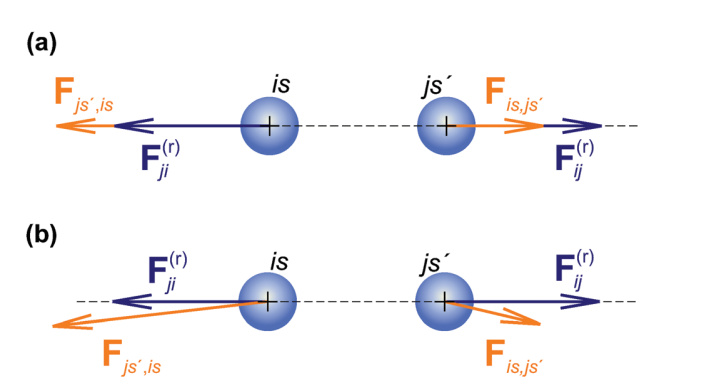
\includegraphics[width=0.7\linewidth]{Ris/1.jpg}}
\caption{Отклонение от третьего закона Ньютона: а) скалярная невзаимность, (б) тензорная 
невзаимность.}
\label{Ivlev}
\end{figure}

Пусть силы действия и взаимодействия действуют вдоль радиус-вектора между
взаимодействующими частицами, но имеют разные величины, как
проиллюстрировано на рис. \ref{Ivlev}.  Тогда $\textbf{F}_{js',is} = F_{js,is} (\textbf{r}_{js'} - \textbf{r}_{is})/|\textbf{r}_{js'} - \textbf{r}_{is}|$ и, следовательно, можно написать

\begin{equation}\label{second}
    F_{js',is} = (1 + \Delta_{s's})F^{(r)}_{ji},
\end{equation}


\begin{equation}\label{third}
    F^{(r)}_{ji} = 1/2(F_{js',is} + F_{is, js'}), ~\Delta_{s's} = \frac{F_{js',is} - F_{is, js'}}{F_{js',is} + F_{is, js'}},
\end{equation}


где $F^{(r)}_{ji}$ - невзаимная часть взаимодействия,  $\Delta_{s's} = - \Delta_{ss'}$ - скалярная характеристика невзаимности, характеризующая видимое отклонение от третьего закона Ньютона, которая, в целом, зависит от расстояния между частицами. Силы $\textbf{F}^{(r)}_{ji}$ подчиняются третьему закону Ньютона для эффективного
взаимодействия и, следовательно, потенциальную энергию $\varphi(r_{ji})$ можно ввести так, чтобы выполнялось $\textbf{F}^{(r)}_{ji} = -\partial \varphi(r_{ji})/\partial \textbf{r}_i$. Можно обеспечить детальную симметрию действие-реакция между каждой парой частиц в подсистемах $s'$ и $s$ за счет перенормировки константы:

\begin{equation}\label{norm}
    \alpha F_{js',is} = \alpha_{s'} F_{is, js'}
\end{equation}


Данный подход эквивалентен перенормировке масс и потенциалов взаимодействия.
Видно, что в случае скалярной радиально независимой
невзаимности, уравнение (\ref{norm}) выполняется в том случае, если силы можно разложить следующим образом:

\begin{equation}\label{force}
    F_{js', is} = f(p_{s'}) g(p_{s}, p_{s'}) F_{ji}^{(r)},
\end{equation}
где $f(p)$ -- произвольная функция параметра $p$,
а $g(p_s, p_{s'}) = g(p_{s'}, p_s)$ 
-- произвольная функция, инвариантная относительно
транспонирования переменных. Параметр $p_s$ вводится для подсистемы $r$, которая связана с невзаимными взаимодействиями: $p_s$ может быть вертикальной координатой слоев частиц
в случае комплексной (пылевой) плазмы или отношением $k/\mu$ химической активности $k$ к подвижности $\mu$ в каталитически активных коллоидах.\\

Используя уравнение (\ref{force}), можно получить решение уравнения (\ref{norm}):

\begin{equation}\label{sixth}
    \alpha_s = A f(p_s), ~\Delta_{s's} = \frac{f(p_{s'}) - f(p_s)}{f(p_{s'}) + f(p_s)}
\end{equation}

где $A$ -- произвольная постоянная. 
Решение означает, что если силы $F_{js',is}$
могут быть представлены
в форме (\ref{force}), то система обладает консервативной (псевдогамильтоновой) динамикой и может быть строго описана в терминах
равновесной статистической механики. Константы $\alpha_s$ определяют температуры подсистем, $T_s  = \alpha_s \widetilde{T}$, где $\widetilde{T}$
является псевдотемпературой, соответствующей перенормированной функции Гамильтона.\\




\section{Невзаимные взаимодействия в пылевой (комплексной) плазме}

В пылевой (комплексной) плазме заряженные микрочастицы левитируют в слабоионизированном газе, например в плазме емкостно связанного радиочастотного разряда. Благодаря взаимодействию гравитационных и электрических сил частицы могут образовывать однослойные или многослойные структуры, в зависимости от условий эксперимента. На взаимодействие между микрочастицами обычно влияет вертикальный поток плазмы, который генерирует так называемые "плазменные вейки" ниже по потоку от каждой частицы. 
Появление плазменных вейков приводит к невзаимности эффективного взаимодействия ~\cite{QYeandFLu}, которое зависит от параметров плазменного разряда и может быть настроено в экспериментах. В результате микрочастицы могут получать энергию из потока плазмы, что открывает широкие перспективы для исследования неравновесных явлений в системах с активационным тепловым поведением, в частности, распространение фронтов пламени,  критических тепловых явлений и термоакустическая неустойчивость в химически активных средах.

Комплексная плазма часто встречается в
космосе. Она присутствует в кольцах планет, хвостах комет, межпланетных
и межзвездных облаках ~\cite{doi:10.1029/RG027i002p00271, Tsytovich_1997}, встречается в окрестностях искусственных
спутников и космических станций ~\cite{Whipple_1981} и др. Также активно исследуется пылевая
плазма в лабораториях.


\begin{figure}[htbp]
\begin{center}
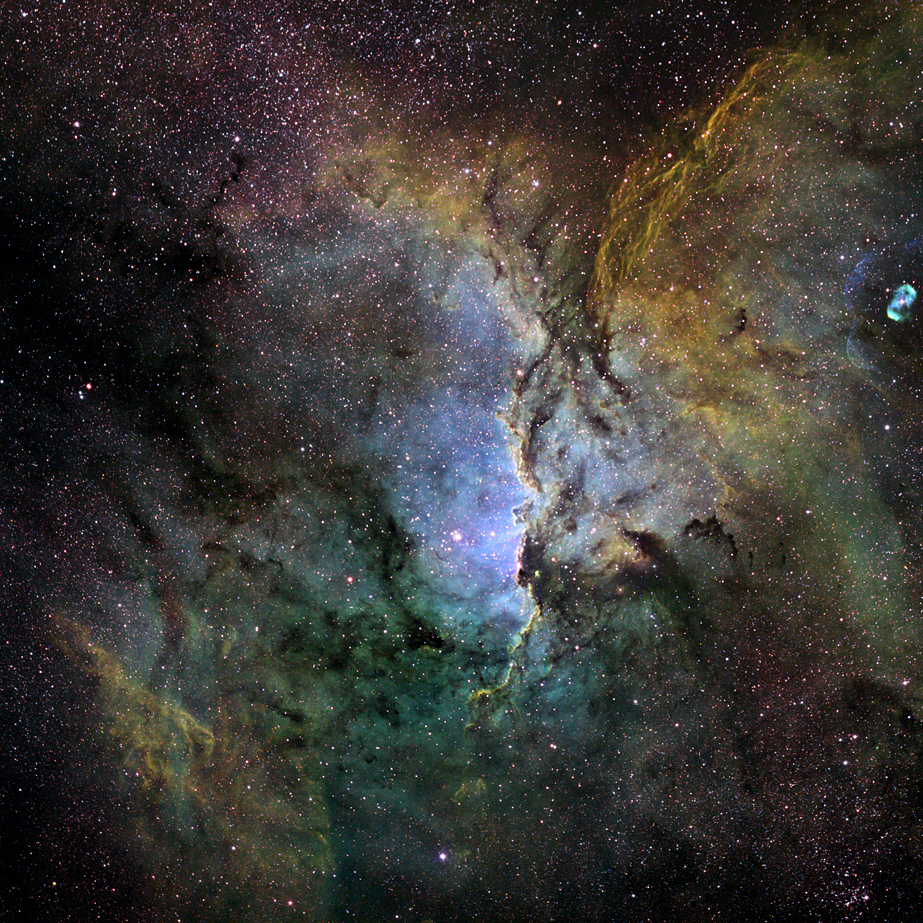
\includegraphics[width=0.3\textwidth]{Ris/8.jpg} ~~ 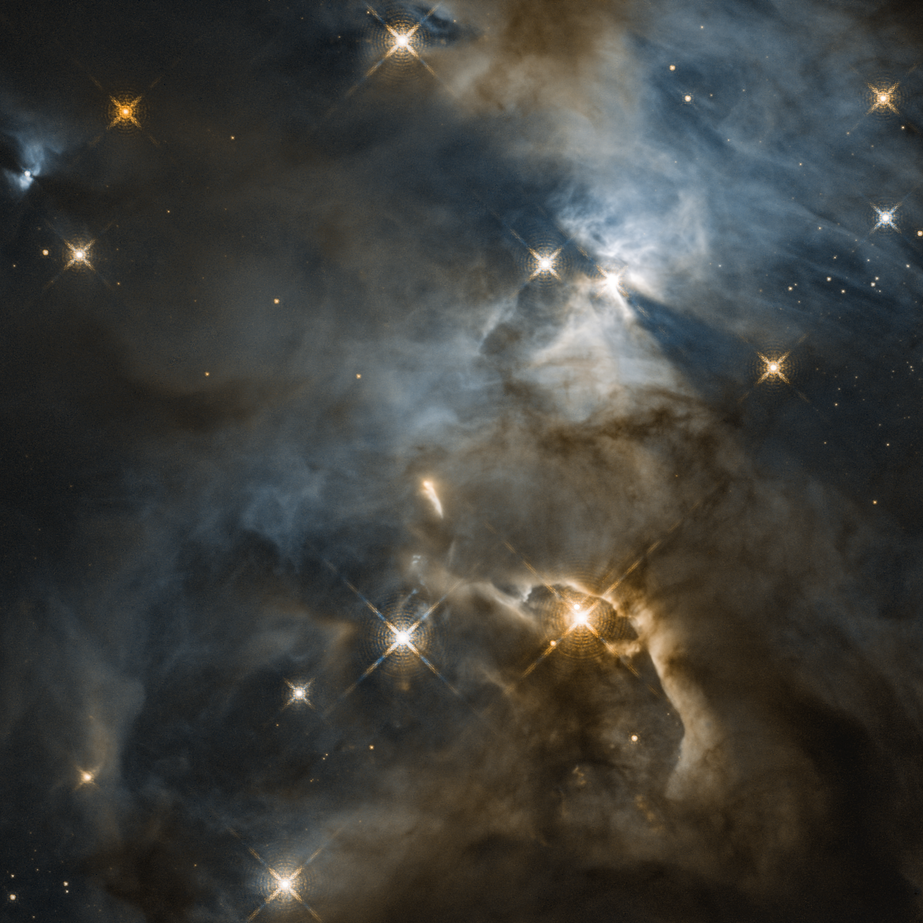
\includegraphics[width=0.3\textwidth]{Ris/6.png} ~~ 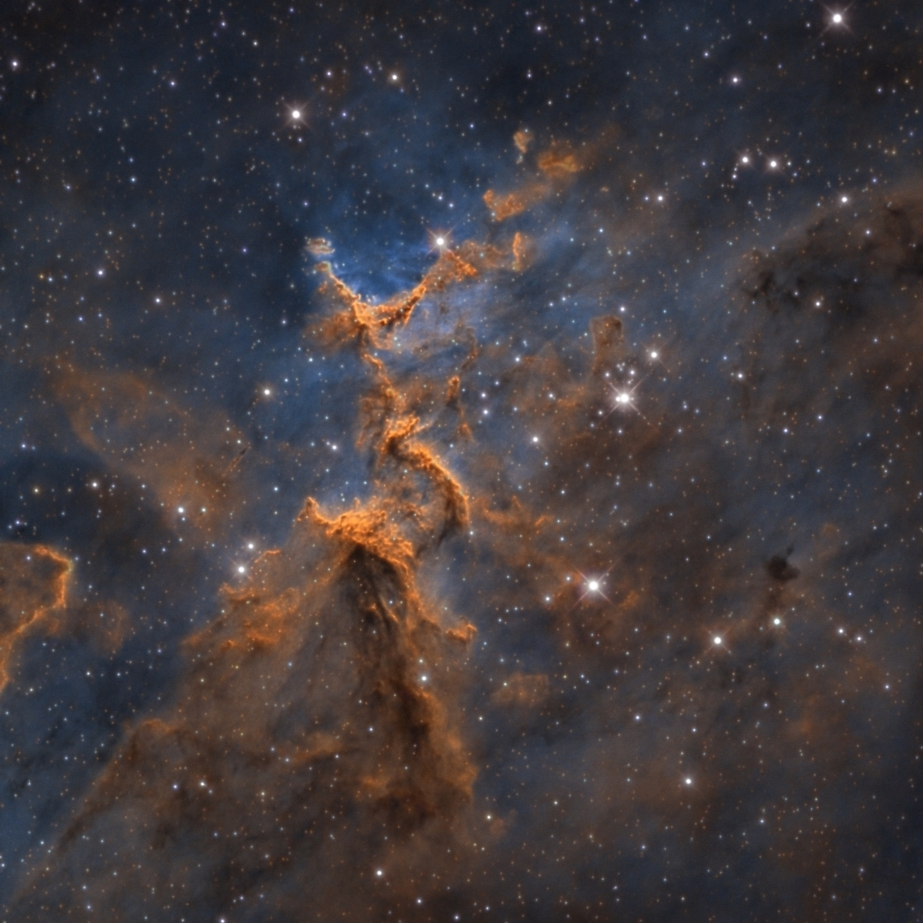
\includegraphics[width=0.3\textwidth]{Ris/7.jpg}
\caption{Пример межзвездных облаков.}
\label{NonRec}
\end{center}
\end{figure}


Наличие массивных заряженных частиц в комплексной плазме имеет
важное значение для коллективных процессов. Ансамбли микрочастиц рождают
новые низкочастотные волновые моды, которые представляют из себя
колебания частиц относительно квазиравновесного фона из электронов
и ионов. Сами частицы достаточно велики, что их можно визуализировать
индивидуально и, следовательно, их движение можно легко отследить. Это
позволяет исследовать явления, происходящие в комплексной плазме на фундаментальном
кинетическом уровене. Частицы микронных размеров, внедренные
в плазму, не только изменяют состав заряда, но и создают новые
физические процессы в системе, например эффекты, связанные с диссипацией
и рекомбинацией плазмы на поверхностях, изменением зарядов частиц и так далее. Эти процессы предполагают новые механизмы притока энергии в систему.
Следовательно, комплексная плазма является новым типом негамильтоновых
систем со свойствами, которые могут полностью отличаться от обычной
многокомпонентной плазмы.

В экспериментальных условиях микрочастицы находятся в условиях конфайнмента
созданного электрическими и гравитационными полями и могут
образовывать в зависимости от условий однослойные или многослойные структуры.
Взаимодействие между микрочастицами обычно зависит от вертикального
потока плазмы, который генерирует так называемые плазменные следы под каждой частицей (рис. \ref{NonRec}).

\begin{figure}[htbp]
\begin{center}
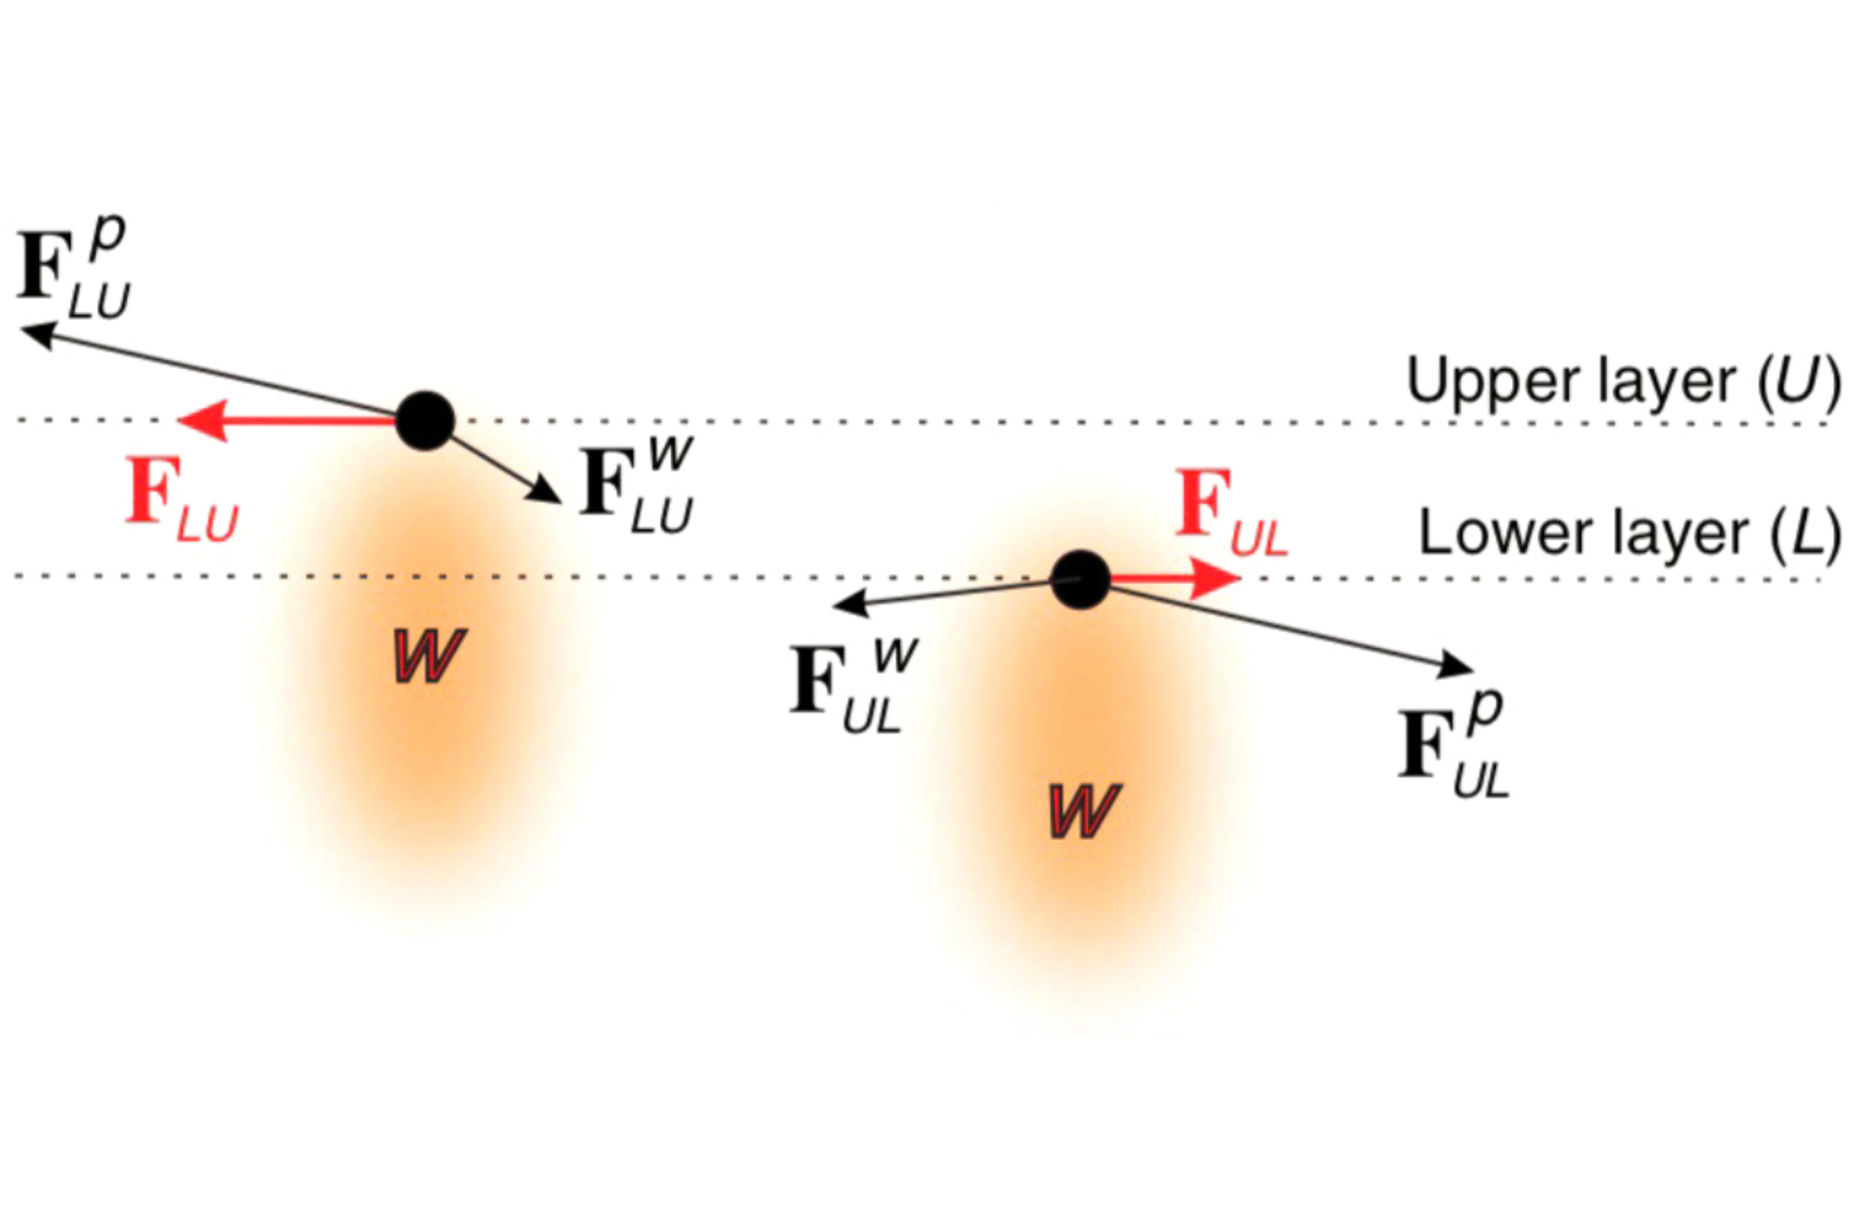
\includegraphics[width=0.7\textwidth]{Ris/wakes2.pdf}
\caption{ Полная сила, действующая на частицу верхнего слоя (U) от частицы нижнего слоя (L).}
\label{NonRec}
\end{center}
\end{figure}


Полная сила, действующая на частицу верхнего слоя (U) от частицы нижнего слоя (L), представляет собой сумму силы отталкивания $\textbf{F}^p_{LU}$ прямого межчастичного взаимодействия и силы притяжения $\textbf{F}^p_{LU}$ от следа нижней частицы (аналогично для полной силы на нижнюю частицу). 

Эффект возникновения плазменных следов приводит к невзаимности
эффективных взаимодействий ~\cite{PhysRevLett.83.3194}, которые зависят от параметров плазменного разряда. В результате, микрочастицы могут получать энергию из плазменного
потока. Данный эффект позволяет исследовать огромный ряд различных
неравновесных явлений: системы с активацией теплового поведения,
в частности, распространение фронтов пламени, ~\cite{PhysRevE.96.043201} критические тепловые
явления ~\cite{PhysRevE.97.043206} и термоакустическая нестабильность в химически реактивных
средах ~\cite{PhysRevLett.121.075003}.


\section{Цели и задачи работы}

\textbf{Цель бакалаврской работы}: 

%Основу для решения указанных задач представляет современный аппарат статистической физики, вычислительной физики и физики конденсированного состояния.